% ------------------------------------------------------------------------------
% TYPO3 Version 10.1 - What's New (Serbian Version)
%
% @license	Creative Commons BY-NC-SA 3.0
% @link		http://typo3.org/download/release-notes/whats-new/
% @language	Serbian
% ------------------------------------------------------------------------------

\section{Izmene za integratore}
\begin{frame}[fragile]
	\frametitle{Izmene za integratore}

	\begin{center}\huge{Poglavlje 2:}\end{center}
	\begin{center}\huge{\color{typo3darkgrey}\textbf{Izmene za integratore}}\end{center}

\end{frame}

% ------------------------------------------------------------------------------
% Feature | 89102 | Read settings for sites from <config>/sites/<siteIdentifier>/settings.yaml
%
%\begin{frame}[fragile]
%	\frametitle{Izmene za integratore}
%	\framesubtitle{Site-specific Settings (1)}
%
%	% decrease font size for code listing
%	\lstset{basicstyle=\smaller\ttfamily}
%
%	\begin{itemize}
%		\item A YAML file can provide site specific variables independent of the current context.
%
%		\item Place the file in the site configuration folder:\newline
%			\texttt{<config>/sites/<siteIdentifier>/settings.yaml}
%
%		\item For example:
%
%\begin{lstlisting}
%Vendor:
%   MyExtension:
%      storagePid: 1
%      limit: 15
%\end{lstlisting}
%
%	\end{itemize}
%
%\end{frame}
%
% ------------------------------------------------------------------------------
% Feature | 89102 | Read settings for sites from <config>/sites/<siteIdentifier>/settings.yaml
%
%\begin{frame}[fragile]
%	\frametitle{Izmene za integratore}
%	\framesubtitle{Site-specific Settings (2)}
%
%	% decrease font size for code listing
%	\lstset{basicstyle=\smaller\ttfamily}
%
%	\begin{itemize}
%		\item Settings can be accessed in TypoScript:
%
%\begin{lstlisting}
%plugin.tx_example.storagePid = {$Vendor.MyExtension.storagePid}
%\end{lstlisting}
%
%		\item Settings can also be accessed in PHP using the \texttt{Site} object:
%
%\begin{lstlisting}
%$settings = $site->getSettings();
%$storagePid = $settings['MyVendor']['MyExtension']['storagePid'];
%\end{lstlisting}
%
%	\end{itemize}
%
%\end{frame}

% ------------------------------------------------------------------------------
% Feature | 89227 | Ask for email address while installing TYPO3

\begin{frame}[fragile]
	\frametitle{Izmene za integratore}
	\framesubtitle{Email adresa administratora}

	\begin{columns}[T]
		\begin{column}{.04\textwidth}
		\end{column}
		\begin{column}{.38\textwidth}

			U toku procesa instalacije, sada se može uneti i email adresa.
			Ova adresa se koristi za inicijalnog korisnika administratorskog interfejsa.

			\vspace{0.2cm}

			Ova opcija postoji i u Maintenance modulu Install Tool-a
			\textbf{Create Administrative User}.

		\end{column}
		\begin{column}{.58\textwidth}
			\vspace{-0.3cm}
			\begin{figure}
				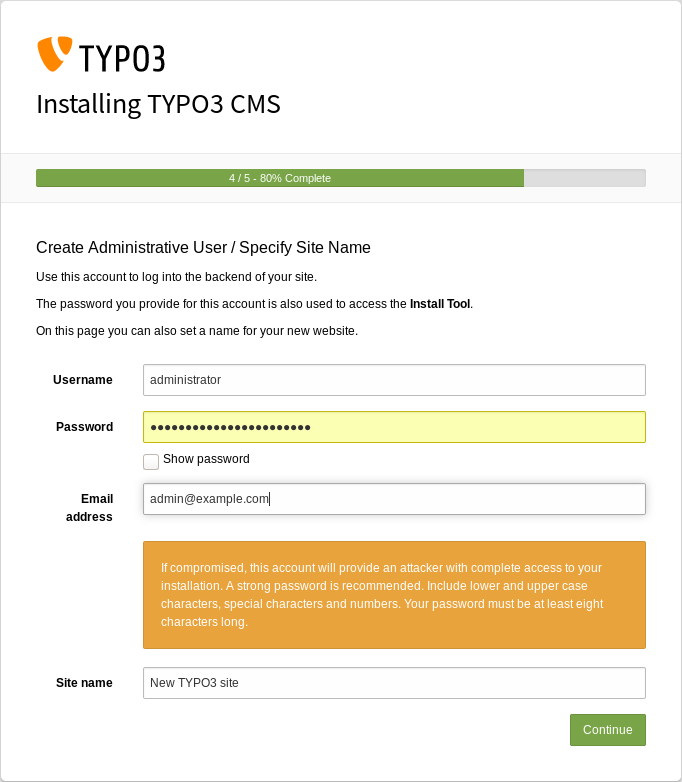
\includegraphics[width=0.70\linewidth]{ChangesForIntegrators/89227-EmailAddressDuringInstallation.png}
			\end{figure}
		\end{column}
	\end{columns}

\end{frame}

% ------------------------------------------------------------------------------
% Feature | 89229 | Cache Preset for Settings in Maintenance Area

% TRANSLATORS, PLEASE BE AWARE:
% We already included this slide in the 10.0 What's New Slides! However, the
% feature #89229 was removed from the TYPO3 core shortly before version 10.0 was
% published. Therefore, you possibly don't need to translate this slide again
% (just copy the text from the previous What's New Slides (search for the term
% "Cache Storage Type" in file ChangesForIntegrators.tex).

\begin{frame}[fragile]
	\frametitle{Izmene za integratore}
	\framesubtitle{Cache Storage Type (1)}

	\begin{itemize}

		\item TYPO3 poseduje fleksibilan sistem keširanja sa podrazumevanim podešavanjima
			i ovo je idealno za većinu slučajeva.
		\item Tip skladišta se sada može podesiti da se fino podesiti keš i povećaju
			performanse u zavisnosti od okruženja.

			\begin{itemize}
				\item Izaberite \textbf{database} skladište za standardna okruženja ili ako se
				 	koristi network file system (NFS).
				\item Izaberite \textbf{file system} ako se koristi sistem sa podeljenim
					bazama podataka
				\item Izaberite \textbf{custom cache settings} da podesite skladište za svaki
					keš posebno.
			\end{itemize}

		\item Za kompleksnije instalacije treba uzeti u obzir memory-based keš kao što je
			\href{https://redis.io/}{Redis}
			ili
			\href{https://memcached.org/}{Memcached}.

	\end{itemize}

\end{frame}

% ------------------------------------------------------------------------------
% Feature | 89229 | Cache Preset for Settings in Maintenance Area

% TRANSLATORS, PLEASE BE AWARE:
% We already included this slide in the 10.0 What's New Slides! However, the
% feature #89229 was removed from the TYPO3 core shortly before version 10.0 was
% published.
%
% On this slide, the path to the function in the backend needs to be adjusted:
% ADMIN TOOLS -> Settings -> Configuration Presets

\begin{frame}[fragile]
	\frametitle{Izmene za integratore}
	\framesubtitle{Cache Storage Type (2)}

	\begin{itemize}

		\item Administratorski interfejs: \textbf{ADMIN TOOLS} \ding{223}\hspace{0.1cm}\textbf{Settings} \ding{223}\hspace{0.1cm}\textbf{Configuration Presets}:
		\end{itemize}

	\begin{figure}
		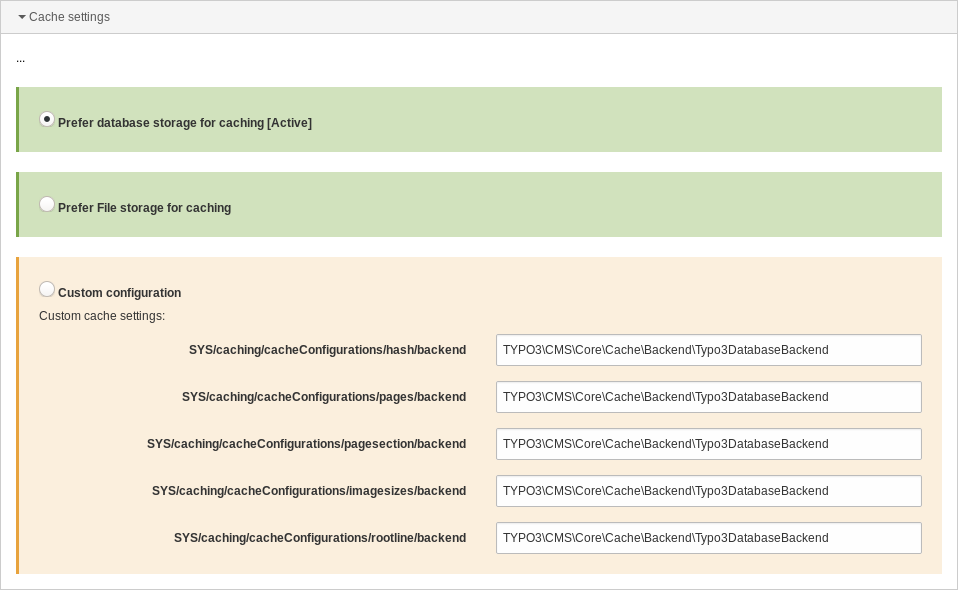
\includegraphics[width=0.60\linewidth]{ChangesForIntegrators/89229-CachePresetForSettingsInMaintenanceArea.png}
	\end{figure}

\end{frame}

% ------------------------------------------------------------------------------
% Feature | 89142 | Create site configuration if page is created on root level

\begin{frame}[fragile]
	\frametitle{Izmene za integratore}
	\framesubtitle{Konfiguracija sajta}

	\begin{itemize}
		\item Kada se napravi nova stranica u korenu sajta, automatski se za nju generiše i
			standardna konfiguracija sajta.
		\item Ovo ima za rezultat da se osnovni TYPO3 sajt može postaviti jako brzo.
		\item Konfiguracija sajta sadrži:

			\begin{itemize}
				\item predefinisan identifikator (e.g. \texttt{site-42-a1d0c6e83f})
				\item ulaznu tačku (e.g. \texttt{https://example.com/site-42})
				\item podrazumevani jezik (e.g. \texttt{English})
			\end{itemize}

	\end{itemize}

\end{frame}

% ------------------------------------------------------------------------------
% Feature | 89090 | Reports for conflicting redirects

\begin{frame}[fragile]
	\frametitle{Izmene za integratore}
	\framesubtitle{Redirekcije u konfliktu (1)}

	\begin{itemize}
		\item Uvedena je nova Symfony komanda da detektuje redirekcije koje su u konfliktu
		 	sa URL-ovima stranica.
		\item Izvršite komandu u terminalu:\newline
			\smaller
				(opcioni parametar \texttt{-}\texttt{-site} sužava proveru samo na izabrani sajt)
			\normalsize
	\end{itemize}

	\begin{figure}
		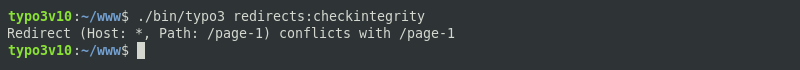
\includegraphics[width=0.90\linewidth]{ChangesForIntegrators/89090a-ReportsForConflictingRedirects.png}
	\end{figure}

	\begin{itemize}
		\item Komanda je dostupna i kao Scheduler task:
	\end{itemize}

	\begin{figure}
		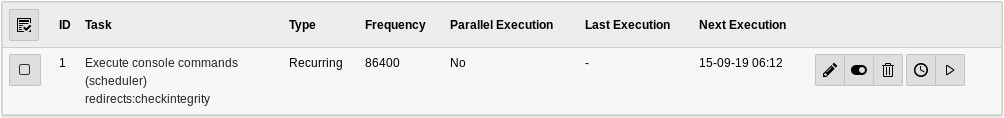
\includegraphics[width=0.90\linewidth]{ChangesForIntegrators/89090b-ReportsForConflictingRedirects.png}
	\end{figure}

\end{frame}

% ------------------------------------------------------------------------------
% Feature | 89090 | Reports for conflicting redirects

\begin{frame}[fragile]
	\frametitle{Izmene za integratore}
	\framesubtitle{Redirekcije u konfliktu (2)}

	\begin{itemize}
		\item Lista svih pronadjenih konfliktnih redirekcija se može videti i u Reports modulu:
	\end{itemize}

	\begin{figure}
		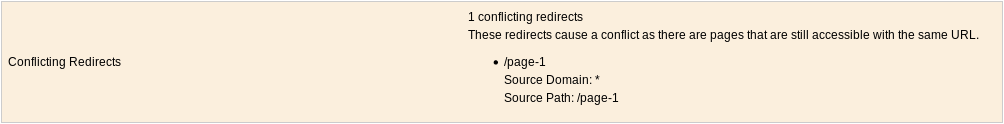
\includegraphics[width=0.90\linewidth]{ChangesForIntegrators/89090c-ReportsForConflictingRedirects.png}
	\end{figure}

	\begin{itemize}
		\item
			\small\textbf{Note:}
				Ova komanda mora da se ponovi da bi se lista ispraznila.
				Rešavanje problema (na primer uklanjanjem redirekcije) neće očistiti listu.
			\normalsize
	\end{itemize}

\end{frame}

% ------------------------------------------------------------------------------
% Feature | 89010 | Introduce Site Configuration for Distribution Packages

\begin{frame}[fragile]
	\frametitle{Izmene za integratore}
	\framesubtitle{Distribuciona pakovanja}

	% decrease font size for code listing
	\lstset{basicstyle=\tiny\ttfamily}

	\begin{itemize}
		\item Distribucije sada mogu da sadrže fajlove konfiguracije sajta.

		\item Kreirajte direktorijum/fajl u distribucionom pakovanju na sledeći način:\newline
			\texttt{Initialisation/Site/<siteIdentifier>/config.yaml}

		\item Slično kao aseti koji se migriraju u \texttt{fileadmin/},\newline
			konfiguracije sajta se migriraju u \texttt{config/} direktorijum.

		\item Ako ovaj direktorijum već postoji, ne vrše se nikakve izmeme postojećih konfiguracija.
	\end{itemize}

\end{frame}

% ------------------------------------------------------------------------------
% Feature | 88318 | Display Application Context in CLI

\begin{frame}[fragile]
	\frametitle{Izmene za integratore}
	\framesubtitle{Kontekst aplikacije u CLI}

	\begin{itemize}
		\item Trenutni kontekst aplikacije se sada prikazuje pored verzije TYPO3-a u
			CLI zahtevima:
	\end{itemize}

	\begin{figure}
		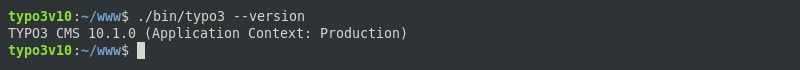
\includegraphics[width=0.90\linewidth]{ChangesForIntegrators/88318-DisplayApplicationContextInCli.png}
	\end{figure}

\end{frame}

% ------------------------------------------------------------------------------
% Feature | 87525 | Add api=1 option in VimeoRenderer

\begin{frame}[fragile]
	\frametitle{Izmene za integratore}
	\framesubtitle{Renderanje Vimeo videa}

	% decrease font size for code listing
	\lstset{basicstyle=\smaller\ttfamily}

	\begin{itemize}
		\item Parametar \texttt{api=1} u Vimeo video URL-u omogućava API interakcije
			sa video plejerom (na primer dodavanje dugmadi za kontrolu videa).
		\item Integratori mogu da postave ovaj parametar sada na dva različita načina.

		\begin{itemize}
			\item Korišćenjem TypoScript-a:

\begin{lstlisting}
lib.contentElement.settings.media.additionalConfig.api = 1
\end{lstlisting}

			\item U Fluid-u korišćenjem Media-ViewHelper:

\begin{lstlisting}
<f:media
  file="{file}"
  alt="{file.properties.alternative}"
  title="{file.properties.title}"
  additionalConfig="{api: 1}"
/>
\end{lstlisting}

		\end{itemize}
	\end{itemize}

\end{frame}

% ------------------------------------------------------------------------------
% Feature | 86670 | Make default action in DragUploader adjustable

\begin{frame}[fragile]
	\frametitle{Izmene za integratore}
	\framesubtitle{Otpremanje fajlova}

	% decrease font size for code listing
	\lstset{basicstyle=\smaller\ttfamily}

	\begin{itemize}
		\item Sada mogu da se konfigurišu podrazumevane akcije kada se otpremaju fajlovi
		u file list modulu korišćenjem drag'n drop.
		\item User TSConfig:

\begin{lstlisting}
# Set default to replace:
options.file_list.uploader.defaultAction = replace

# Set default to rename:
options.file_list.uploader.defaultAction = rename

# Set default to cancel:
options.file_list.uploader.defaultAction = cancel
\end{lstlisting}

	\end{itemize}

\end{frame}

% ------------------------------------------------------------------------------
% Feature | 84250 | Separately enable / disable "Add media by URL" and "Select & upload files"

\begin{frame}[fragile]
	\frametitle{Izmene za integratore}
	\framesubtitle{Dugmad za Media Element}

	% decrease font size for code listing
	\lstset{basicstyle=\tiny\ttfamily}

	\begin{itemize}
		\item Dugmad \textbf{"Add media by URL"} i \textbf{"Select \& upload files"}
			 sada mogu da se omoguće/onemoguće nezavisno jedno od drugog.
	\end{itemize}

	\begin{figure}
		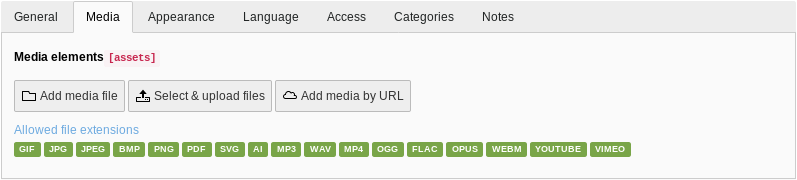
\includegraphics[width=0.75\linewidth]{ChangesForIntegrators/84250-EnableDisableMediaButtons.png}
	\end{figure}

	\begin{itemize}
		\item Sledeći primer onemogučuje oba dugmeta:

\begin{lstlisting}
$GLOBALS['TCA']['pages']['columns']['media']['config']['appearance'] = [
  'fileUploadAllowed' => false,
  'fileByUrlAllowed' => false,
];
\end{lstlisting}

	\end{itemize}

\end{frame}

% ------------------------------------------------------------------------------
% Feature | 88441 | Show configuration of USER_INT objects in adminpanel

\begin{frame}[fragile]
	\frametitle{Izmene za integratore}
	\framesubtitle{Admin Panel}

	\begin{itemize}
		\item Admin Panel sada ima novi panel \textbf{USER\_INT} u "Info" modulu.
	\end{itemize}

	\begin{figure}
		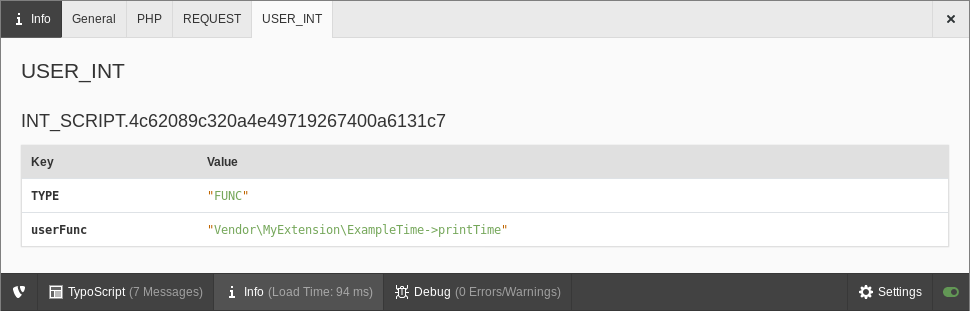
\includegraphics[width=0.90\linewidth]{ChangesForIntegrators/88441-ShowUserIntObjectsInAdminPanel.png}
	\end{figure}

\end{frame}

% ------------------------------------------------------------------------------
